\documentclass[../TST.tex]{subfiles}
\begin{document}
\begin{pproblem}
A monochromator consists of:
\begin{itemize}[nosep, label=--]
	\item An isosceles glass prism of base $b=\qty{10.0}{cm}$ and an angle $\theta=\ang{50}$ opposite the base.
	\item A thin entrance slit.
	\item An identical exit slit.
	\item A lens at the entrance which gives rise to a parallel beam incident on the prism.
	\item An identical lens which focuses the dispersed light onto the exit slit. The lenses are of diameter $D=\qty{10.0}{cm}$ and focal length $f=\qty{50.0}{cm}$.
\end{itemize}
The glass of the prism has a refractive index $n=1.73$. Its dispersion at wavelength 550 nm is $\frac{\mathrm{d}n}{\mathrm{d}\lambda}=\qty{1.35e5}{m^{-1}}$. Inside the prism light travels parallel to the base. Using the Rayleigh criterion, find the theoretical upper limit for the spectral resolution of the monochromator $R=\lambda/\Delta \lambda$ (due to diffraction). Calculate $R$.
\end{pproblem}

\ifprob \else
	\begin{solution} This is quite tough, and we should try to get our head around it using a diagram. First, the entrance slit has to be positioned at the focus of the first lens. This ensures that all the light that emerges from the slit will come out as a parallel beam of diameter $D$. The beam is then incident on the prism, with the angle of incidence $\alpha$ set up so that the rays will be parallel to the base of the prism following their refraction. The angle of refraction should be equal to $\theta/2$ for this to happen, so the angle of incidence can be found from  $\sin\alpha= n\sin{(\theta/2)}$. Upon leaving the prism, the rays undergo refraction a second time, and come out as a parallel beam by symmetry. This beam is incident on the second lens, which focuses it onto a single point in its focal plane. This is where the exit slit is.\\[5pt]
		So far we have outlined how the prism works at a fixed wavelength, say $\lambda_0 =\qty{550}{nm}$. However, the prism's refractive index varies with $\lambda$, and light whose wavelength is shifted from $\lambda_0$ by some $\Delta\lambda$ will encounter a refractive index shifted by $\Delta n = \frac{\mathrm{d}n}{\mathrm{d}\lambda}\Delta\lambda$. Such rays will take on a different trajectory, but they will again come out as a parallel beam. Each $\lambda$ will then have its own parallel beam which is focused at a specific point in the focal plane of the second lens. This would imply that all the different wavelengths can be distinguished by their position in the focal plane at the exit slit. Unfortunately, we also have diffraction at the second lens, which means that the focusing is imperfect. Instead of a single point, we get a smeared-out image with a characteristic angular size $\chi\approx 2\lambda/d$, where $d$ is the relevant aperture at the second lens. This can either be the diameter of the lens $D$ or the width of the incident beam $l$, if that's less than $D$ -- we'll need to check this later. Now, according to the Rayleigh criterion, two wavelengths will be indistinguishable if their spots overlap too much, the limit being when the centre of one spot lies on the rim of the other. Let the parallel beams for two distinct wavelengths make an angle $\Delta\beta'$ when they come out of the prism. As we can see from the diagram, the distance between the centres of their spots at the exit slit is $\Delta \beta'f$, while the `radius' of each spot is $\frac{\lambda f}{d}$. Hence, the limiting $\Delta\beta'$ is equal to $\lambda/d$. We will need to express this $\Delta \beta'$ in terms of the wavelength difference $\Delta \lambda$, after which we can write $R=\lambda/\Delta \lambda$, and we're done.\\[5pt]
		\begin{center}
		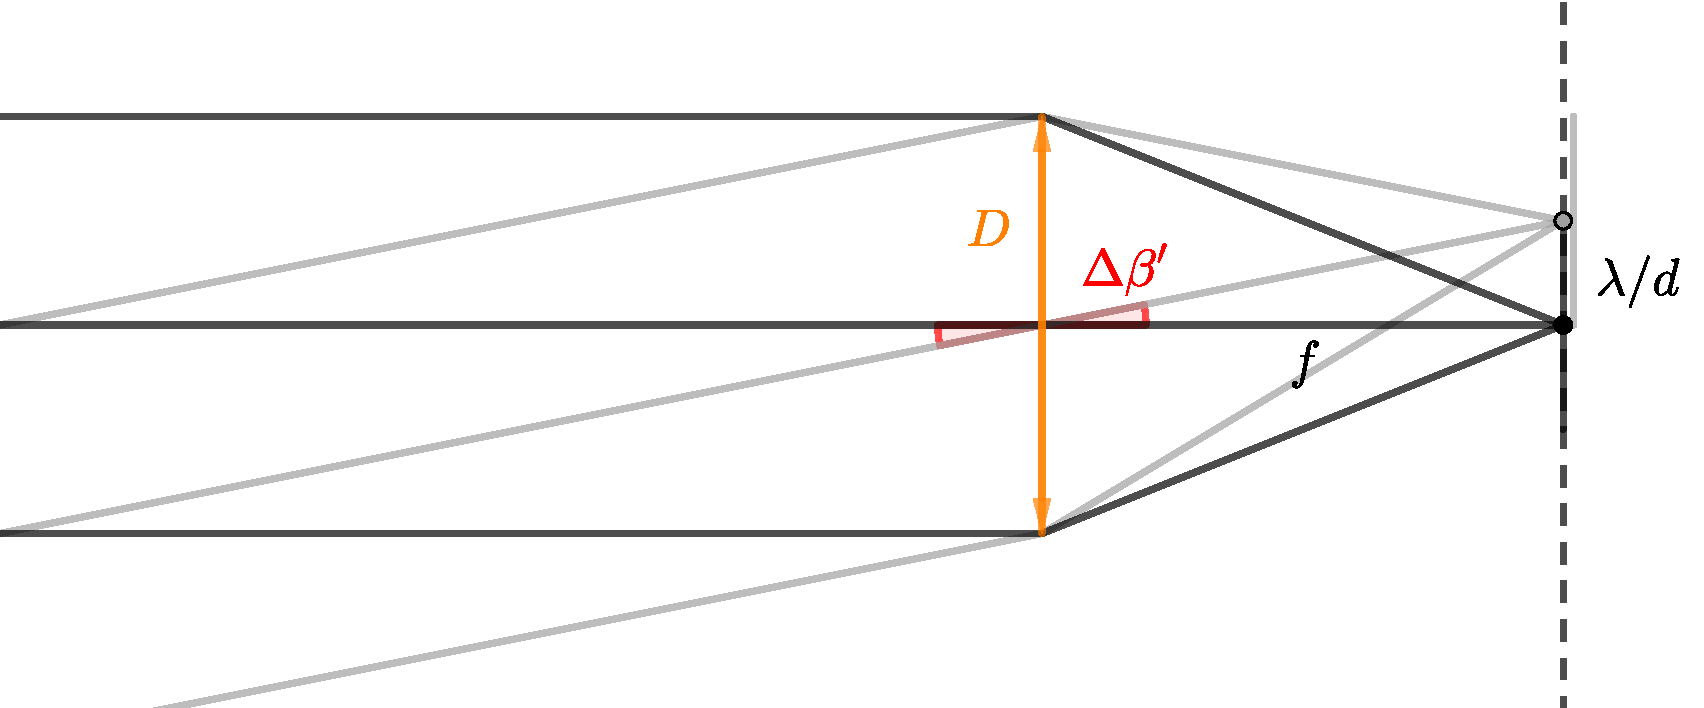
\includegraphics[width=0.8\textwidth]{fig/a2013_s61.pdf}
		\end{center}
		
Consider two rays that diverge due to a difference $\Delta n$ in the refraction index. Since both are incident at the same $\alpha$, we can differentiate Snell's law to find the difference $\Delta \beta$ in their refraction angles, like so:
\begin{equation*}
	n\sin\beta=\sin{\alpha} \quad\Rightarrow\quad \Delta n \sin\beta + n\cos\beta\,\Delta \beta=0 \quad\Rightarrow\quad \Delta \beta = - \frac{\Delta n}{n} \tan{\beta}
.
\end{equation*}
		\begin{center}
		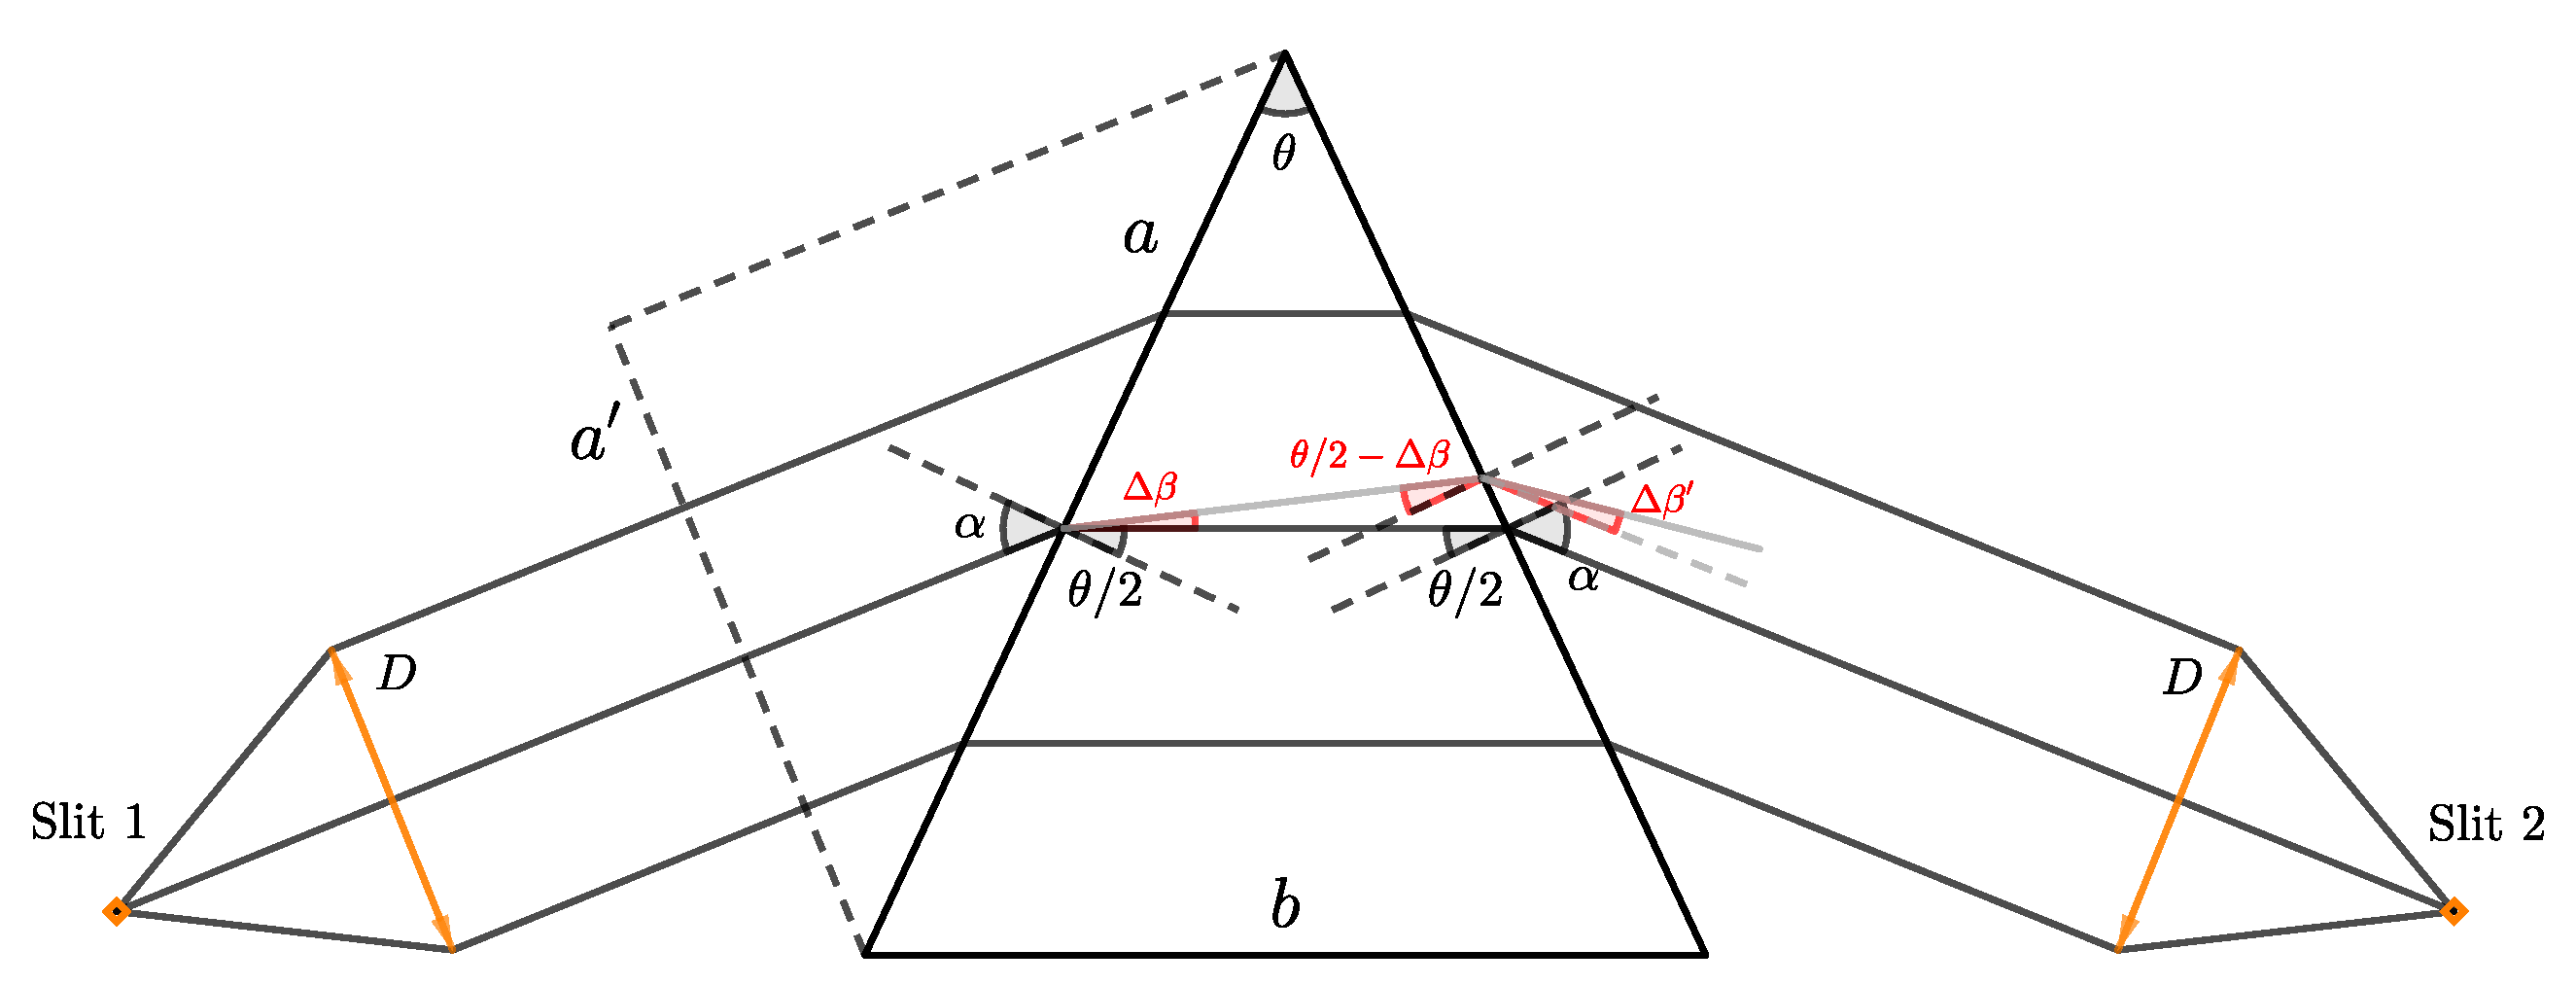
\includegraphics[width=\textwidth]{fig/a2013_s62.pdf}
		\end{center}
When the rays get to the other side of the prism, the difference in their incidence angles is $\Delta \alpha ' =-\Delta \beta$. After they exit the prism, their refraction angles will differ by some $\Delta \beta'$ which can be obtained from Snell's law. This time around we need to be careful, since both the incidence angle and the refractive index will vary:
\begin{equation*}
	n\sin\alpha'=\sin{\beta'} \quad\Rightarrow\quad \Delta n \sin\alpha' + n\cos\alpha'\,\Delta \alpha'=\cos{\beta'}\Delta \beta'
\end{equation*}
Now we can substitute $\alpha'= \beta = \frac{\theta}{2}$. After plugging in our expression for $\Delta\beta$, the left hand side adds up to $2\Delta n \sin{\frac{\theta}{2}}$. As for the right hand side, we can use $\beta'=\alpha$ and $\cos{\alpha}=\sqrt{1-\sin^2{\alpha}}=\sqrt{1-n^2\sin^2\left(\frac{\theta}{2}\right)}$. Then we have
\begin{equation*}
	\Delta\beta'=\frac{2\sin\!{\left(\frac{\theta}{2}\right)\left( \frac{\mathrm{d}n}{\mathrm{d}\lambda}\right)\Delta\lambda}}{\sqrt{1-n^2\sin^2\left(\frac{\theta}{2}\right) }}
.
\end{equation*}
Next, let's figure out the aperture $d$. The legs of the prism have length $a=\frac{b/2}{\sin{(\theta/2)}} $, and their projection perpendicular to the incident beam is 
\begin{equation*}
	a'=a\cos{\alpha}=\frac{b}{2\sin{\left(\frac{\theta}{2}\right)}}\sqrt{1-n^2\sin^2\left(\frac{\theta}{2}\right) }=\qty{8.1}{cm}.
\end{equation*}
This is less than $D=\qty{10.0}{cm}$, so the transmitted beam's cross-section will be limited to $a'$ along some direction. The effective aperture is then $d=a'$. Therefore,
\begin{equation*}
	R=\frac{\lambda}{\Delta \lambda}= \frac{\Delta\beta' d}{\Delta \lambda}=\frac{\Delta\beta' a'}{\Delta \lambda} = \boxed{b \frac{\mathrm{d}n}{\mathrm{d}\lambda}=13500.}
\end{equation*}
Note that we have diffraction at the first lens and at the prism as well, but this doesn't matter much by the time we get to the second lens. For a similar problem about dispersion, see RMPh 2017-1A.
\end{solution}
\fi

\end{document}
